\section{Endpoint square summation and the order of limits}
\label{sec:endpoint}

The exponent $p>2$ in Theorem~\ref{thm:distribution} has a final, essential
use. It supplies a positive convexity deficit on a common dyadic time
tree. Combined with spatial localization, this gives a square sum over
frequency scales and hence the Sobolev norm at the endpoint.  We then construct a representative continuous in time
and verify that the prescribed Gaussian limits recover that representative
at every real time on one full-measure set.

Throughout this section, $S(t)f=e^{it\Delta}f$ denotes the $L^2$ evolution,
whose Fourier multiplier is $e^{-it|\xi|^2}$.  When $\widehat f$ has compact
support, we also use $S(t)f(x)$ for its absolutely convergent Fourier
integral.  This is continuous in $(x,t)$, since then
$\widehat f\in L^1$.  Constants may depend on fixed annular supports and
smooth cutoff functions, but are independent of frequency, the center of
a spatial ball, and every measurable choice of time made below.

\subsection{From packet distributions to a short-time maximal estimate}

For $p>0$ and measurable $h$ on $A\subset\R^2$, we use the weak $L^p$
quasinorm
\[
 \|h\|_{L^{p,\infty}(A)}
   =\sup_{\lambda>0}\lambda
      |\{x\in A:|h(x)|>\lambda\}|^{1/p}.
\]

\begin{proposition}[Short-time maximal estimate]
\label{prop:shortmax}
Let $p>2$ be the exponent in Theorem~\ref{thm:distribution}.  Fix
$0<c_0<C_0<\infty$.  If $N\ge1$ is dyadic and
\[
 \supp\widehat f_N\subset
 \{\xi\in\R^2:c_0N\le |\xi|\le C_0N\},
\]
then, on every unit ball $B\subset\R^2$,
\begin{equation}
 \left\|\sup_{0<t<1/N}|S(t)f_N|\right\|_{L^{p,\infty}(B)}
 \le C N^{1/3}\|f_N\|_2.
 \label{eq:src24}
\end{equation}
The same estimate holds on every translated time interval of length at
most $1/N$, with either endpoint included.
\end{proposition}

\begin{proof}
We first apply Theorem~\ref{thm:distribution} at $D=1$ to an arbitrary
measurable spatial graph in unit-frequency variables.  Let
$\mathcal B$ be a spatial ball of radius $O(L^2)$, let
$T:\mathcal B\to[0,L^2]$ be measurable, and define
\begin{equation}
 \mu(F)=\int_{\mathcal B}{\bf1}_F(X,T(X))\,dX.
 \label{eq:endpoint-graph-measure}
\end{equation}
This is the pushforward of spatial area, regardless of the regularity of
$T$.  A space-time ball of radius $r$ projects into a spatial disk of the
same radius, so $\mu(B_r)\le\pi r^2$.  A tube of width $L$ and time length
$L^2$, with one of the bounded velocities in the packet class, is covered
by $O(L)$ space-time balls of radius $CL$.  Its $\mu$-mass is therefore
$O(L^3)$.  A transverse enlargement by $2^\ell$ can be covered by
$O(L2^{2\ell})$ such balls.  Summing these bounds against the decay
$2^{-M\ell}$, where $M$ is the fixed large exponent in
\eqref{eq:src6}, proves that condition with $D=1$ after a fixed enlargement
of $m$.  All constants here are uniform over $T$, the packet intercepts,
and the center of $\mathcal B$.

We explain why the compact packet estimate applies to an exact
unit-frequency extension
\[
 Ev(X,T)=\int e^{i(X\cdot\eta-T|\eta|^2)}v(\eta)\,d\eta,
 \qquad \supp v\subset\{c_0\le |\eta|\le C_0\}.
\]
Apply Lemma~\ref{lem:packets} at packet width $L$.  It gives
$v=\sum_{\omega,n}c_{\omega,n}v_{\omega,n}$, with
$\omega\in L^{-1}\mathbb Z^2$, $n\in\mathbb Z^2$, and
\[
 \sum_{\omega,n}|c_{\omega,n}|^2\le C\|v\|_2^2.
\]
Its exact profile formula \eqref{eq:prelim-exact-profile} reads
\[
\begin{gathered}
 Ev_{\omega,n}(X,T)
 =L^{-1}e^{i(X\cdot\omega-T|\omega|^2)}
 H\left(\frac{X-Ln-2\omega T}{L},\frac{T}{L^2}\right),
 \\[2pt]
 H(z,s)=\frac1{2\pi}\int\psi(\zeta)
                   e^{i(z\cdot\zeta-s|\zeta|^2)}\,d\zeta,
\end{gathered}
\]
where $\psi$ is the fixed smooth frequency cutoff in that lemma.
The phase-space counts are bounded, and, on every fixed bounded
$s$-interval, all required derivatives of $H$ decrease faster than
any fixed power of $|z|$.  The remaining issue is its noncompact
spatial support; we resolve it by summing compact layers.

To obtain the compact profiles of \eqref{eq:src5}, choose a smooth time
cutoff equal to one on $[0,1]$, and a spatial partition of unity
$\sum_{q\in\mathbb Z^2}\rho(z-q)=1$ with $\rho$ compactly supported.
Fix the finite profile derivative order required by
Theorem~\ref{thm:distribution}.  In the $q$th term replace the intercept $Ln$ by
$Ln+Lq$.  The new profile is the old profile evaluated at
$z+q$, multiplied by $\rho(z)$ and the time cutoff.  For any prescribed
large $A$, its required derivative bounds are
$O((1+|q|)^{-A})$.  Put this factor into the coefficients.  For each fixed
$q$, all phase-space intercepts undergo the same translation, so the
counting bounds are preserved, and the new coefficient norm is at most
\[
 C_A(1+|q|)^{-A}\|v\|_2.
\]
Thus every layer is an admissible array for Theorem~\ref{thm:distribution}.

The exponent $A$ is chosen once, after the required derivative order;
the fixed profile bound may depend on both, but never on $L$ or $q$.
For completeness, let $b_q>0$ satisfy $\sum_q b_q=1$ and
$b_q\asymp(1+|q|)^{-3}$.  Apply \eqref{eq:src12} to the $q$th layer at
threshold $b_q\lambda$, using homogeneity in its coefficients.  Choosing
$A$ sufficiently large makes
$\sum_q b_q^{-p}(1+|q|)^{-Ap}$ finite and yields
\begin{equation}
 \mu\{|Ev|>\lambda\}
 \le C L^4\bigl(\lambda L^{4/3}\bigr)^{-p}\|v\|_2^p.
 \label{eq:endpoint-exact-weak}
\end{equation}
These operations can first be made on finite packet sums.  At a point,
each frequency label has only $O(1)$ intercepts contributing to a fixed
compact layer, and there are $O(L^2)$ frequency labels.  Cauchy--Schwarz
therefore bounds that layer by $C(1+|q|)^{-A}\|v\|_2$, uniformly in $L$;
the factor $L$ from the square root of the label count cancels the
packet amplitude $L^{-1}$.  The same bound holds with the coefficient
norm of any tail in place of $\|v\|_2$.  Taking $A>2$ makes the layer sum
absolutely and uniformly convergent, and square-summability makes
finite coefficient truncations converge uniformly as well.
Fourier-series partial sums also converge in $L^2$ on a fixed bounded
frequency set, hence their exact extensions converge uniformly by
Cauchy--Schwarz in frequency.  These observations identify the compact
layer sum with the exact extension.  Passing to the limit in the distribution
bound, first with a slightly smaller threshold, proves
\eqref{eq:endpoint-exact-weak} for arbitrary $v\in L^2$ with the indicated
support.  This passage uses exact extensions and therefore introduces no
time-dependent choices of representatives.

Now take $L=\sqrt N$ and
$v(\eta)=N\widehat f_N(N\eta)$.  Then
$\|v\|_2=\|\widehat f_N\|_2$, and
\begin{equation}
 S(t)f_N(x)=(2\pi)^{-2}N\,Ev(Nx,N^2t).
 \label{eq:endpoint-frequency-scaling}
\end{equation}
A unit spatial ball becomes a ball of radius $N=L^2$, and a time interval
of length $1/N$ becomes one of length $N=L^2$.  For a measurable physical
graph $t=t(x)$, its lifted spatial area in the new coordinates is $N^2$
times the original area.  This cancels $L^4$ in
\eqref{eq:endpoint-exact-weak}.  The threshold scale in the physical
field is
\[
 N L^{-4/3}=N^{1/3}.
\]
Consequently, for every such graph and every $\lambda>0$,
\[
 \bigl|\{x\in B:|S(t(x))f_N(x)|>\lambda\}\bigr|
 \le C\left(\frac{N^{1/3}\|f_N\|_2}{\lambda}\right)^p.
\]
For finitely many times choose, measurably, the first time attaining the
largest modulus.  Apply this graph bound, then increase the finite list
to a countable dense set.  Continuity of the bounded-frequency evolution
identifies the resulting supremum with the supremum over all times and
allows the endpoints.  Finally, replacing $f_N$ by $S(t_0)f_N$ translates
the interval without changing either its Fourier support or its $L^2$
norm.
\end{proof}

\subsection{Two dual estimates on a short time interval}

Fix a unit spatial ball $\Omega$, a measurable function
$t:\Omega\to[0,1)$, and a measurable complex function $w$ with $|w|\le1$.
These choices remain the same at every frequency.  For $N=2^j$, $j\ge1$,
let $\chi_N(\xi)=\chi(\xi/N)$ be a smooth cutoff supported on a fixed
annulus away from zero.  The same argument permits finitely many fixed
choices of $\chi$.  For a half-open time interval $I\subset[0,1)$, put
\begin{align}
 E_I&=\{x\in\Omega:t(x)\in I\},
 &m_I&=|E_I|,\notag\\
 G_N(I)(\xi)&=\chi_N(\xi)\int_{E_I}
              w(x)e^{i(x\cdot\xi-t(x)|\xi|^2)}\,dx,
 &e_j(I)&=N^{-2/3}\|G_N(I)\|_2^2.
 \label{eq:endpoint-dual-definitions}
\end{align}
The quantities $m_I$ are the masses of a single measure on time, the
pushforward of ${\bf1}_\Omega dx$ under $t$.  This measure can have atoms;
all interval partitions below are half-open so membership is unique.

We will use the elementary weak-space integration bound
\begin{equation}
 \int_F |h|\le \frac{p}{p-1}
             \|h\|_{L^{p,\infty}}|F|^{1-1/p}.
 \label{eq:endpoint-weak-integration}
\end{equation}
Indeed the layer-cake formula bounds its left side by
$\int_0^\infty\min\{|F|,(\|h\|_{L^{p,\infty}}/\lambda)^p\}\,d\lambda$;
splitting where the two terms agree gives the stated expression.

The kernel for pairings of the dual functions is
\begin{equation}
 K_N(z,\tau)=\int |\chi_N(\xi)|^2
                   e^{i(z\cdot\xi-\tau|\xi|^2)}\,d\xi
 =N^2\int|\chi(\eta)|^2
                   e^{i(Nz\cdot\eta-N^2\tau|\eta|^2)}\,d\eta.
 \label{eq:endpoint-kernel}
\end{equation}
In particular,
\[
 \langle G_N(I),G_N(J)\rangle
 =\int_{E_I}\int_{E_J}w(x)\overline{w(y)}
       K_N(x-y,t(x)-t(y))\,dy\,dx.
\]
Only the smooth frequency variable will be differentiated in estimates
for this kernel.  No regularity of the graph $t(x)$ is needed.

\begin{lemma}[Separation in time]
\label{lem:endpoint-time-separation}
Let $\mathcal D_j$ be the dyadic partition of $[0,1)$ into intervals of
length $2^{-j}=1/N$.  Then
\begin{equation}
 e_j([0,1))\le C\sum_{I\in\mathcal D_j}e_j(I)+CN^{-2}.
 \label{eq:endpoint-time-almost-orthogonality}
\end{equation}
\end{lemma}

\begin{proof}
For two intervals whose indices differ by at most a sufficiently large
fixed integer $C_1$, Hilbert-space Cauchy--Schwarz bounds their pairing by
the geometric mean of their squared norms.  Each interval has only
$O(C_1)$ such neighbors, so their total contribution is at most
$C\sum_I\|G_N(I)\|_2^2$.

For all other pairs, $|t(x)-t(y)|\ge(C_1-1)/N$, while
$|x-y|\le2$.  Write $z=x-y$ and $\tau=t(x)-t(y)$.  On the support of
$\chi$, the gradient
\[
 \nabla_\eta(Nz\cdot\eta-N^2\tau|\eta|^2)
      =Nz-2N^2\tau\eta
\]
has magnitude at least $cN^2|\tau|$ if $C_1$ is large enough, since the
annulus has a positive inner radius.  Dividing the phase by
$N^2|\tau|$ gives a smooth phase with uniformly bounded derivatives and
a uniformly nonvanishing gradient.  Repeated integration by parts gives,
for every fixed integer $M$,
\[
 |K_N(z,\tau)|\le C_M N^2(N^2|\tau|)^{-M}
                 \le C_M N^{2-M}.
\]
Integrate this bound once over the full set of far pairs, whose spatial
measure is at most $|\Omega|^2$.  There is no additional factor for the
number of interval pairs.  After normalization by $N^{-2/3}$, taking
$M=4$ gives an error $O(N^{-8/3})$, which is bounded by $O(N^{-2})$.
\end{proof}

\begin{lemma}[Mass and spatial localization]
\label{lem:endpoint-localized-dual}
If $I\in\mathcal D_j$ and $J\subset I$ is a dyadic descendant at relative
depth $k$, where $0\le k\le j$, set $r=2^{-k}$.  Then
\begin{align}
 e_j(J)&\le C m_J^{2-2/p},
 \label{eq:endpoint-mass-bound}\\
 e_j(J)&\le C r^{2/3}m_J.
 \label{eq:endpoint-spatial-bound}
\end{align}
Consequently, with
\[
 \alpha=\frac32-\frac1p=1+\frac{1-2/p}{2}>1,
\]
we have
\begin{equation}
 e_j(J)\le C2^{-k/3}m_J^\alpha.
 \label{eq:endpoint-interpolated-dual}
\end{equation}
\end{lemma}

\begin{proof}
For the first estimate, dualize the frequency $L^2$ norm in
\eqref{eq:endpoint-dual-definitions}.  Against a frequency test function
of norm one, the spatial integrand is an annular Schr\"odinger extension
with input norm bounded by a fixed constant.  Its values at $t(x)$ are
bounded by its short-time maximal function on the interval $J$, whose
length is at most $1/N$.  Proposition~\ref{prop:shortmax} and
\eqref{eq:endpoint-weak-integration} therefore give
\[
 \|G_N(J)\|_2\le C N^{1/3}m_J^{1-1/p}.
\]
Squaring and normalizing proves \eqref{eq:endpoint-mass-bound}.

For the second estimate, partition space into half-open squares $Q$ of
side $r$, and write $G_N(J,Q)$ for the same dual integral over
$E_J\cap Q$.  Set $m_{J,Q}=|E_J\cap Q|$.  Declare two squares neighbors
if their grid indices differ by at most a sufficiently large fixed
constant $C_2$.  Neighbor interactions are bounded by
$C\sum_Q\|G_N(J,Q)\|_2^2$, using Cauchy--Schwarz and the bounded number of
neighbors of each square.

For non-neighboring squares, $|x-y|\ge cC_2r$, whereas
$|t(x)-t(y)|\le |J|=r/N$.  Choose $C_2$ using the outer radius of the
annular support.  The spatial part now dominates the gradient of the
phase in \eqref{eq:endpoint-kernel}, and integration by parts gives
\[
 |K_N(x-y,t(x)-t(y))|
       \le C N^2(1+N|x-y|)^{-4}.
\]
The right side has a uniformly bounded spatial integral.  Since the
graph measure is projected spatial area and $|w|\le1$, the total
normalized contribution of these far pairs is at most
\begin{equation}
 C N^{-2/3}\int_{E_J}\int_{\R^2}
           N^2(1+N|x-y|)^{-4}\,dy\,dx
 \le C N^{-2/3}m_J\le C r^{2/3}m_J.
 \label{eq:endpoint-spatial-far-error}
\end{equation}
The last inequality is exactly where $k\le j$, equivalently $Nr\ge1$,
is used.

It remains to estimate a single square contribution.  Let $x_Q$ be the
center of $Q$ and $t_J$ the left endpoint of $J$.  Make the change
\[
 x=x_Q+rX,\qquad t=t_J+r^2s,\qquad \xi=\eta/r.
\]
The new graph lies in a unit spatial ball, has spatial area
$r^{-2}m_{J,Q}$, and has times in an interval of length
\[
 \frac{|J|}{r^2}=\frac1{Nr}.
\]
The new annular frequency is $Nr\ge1$.  The dual function acquires the
factor $r^2$ from $dx$ and a unimodular factor from $x_Q,t_J$; changing
frequency measure gives
\[
 \|G_N(J,Q)\|_2^2=r^2\|\widetilde G_{Nr}\|_2^2.
\]
Apply Proposition~\ref{prop:shortmax} and
\eqref{eq:endpoint-weak-integration} directly at the normalized scale,
including its lowest possible value $Nr=1$.  This gives
\begin{align*}
 N^{-2/3}\|G_N(J,Q)\|_2^2
 &\le C N^{-2/3}r^2(Nr)^{2/3}
                     (r^{-2}m_{J,Q})^{2-2/p}\\
 &=C r^{-4/3+4/p}m_{J,Q}^{2-2/p}
 \le C r^{2/3}m_{J,Q},
\end{align*}
where the last step uses $m_{J,Q}\le r^2$ and $2-2/p>1$.
Sum this estimate over $Q$, include the bounded neighbor interactions
and \eqref{eq:endpoint-spatial-far-error}, and obtain
\eqref{eq:endpoint-spatial-bound}.  Finally, the geometric mean of
\eqref{eq:endpoint-mass-bound} and \eqref{eq:endpoint-spatial-bound} is
\eqref{eq:endpoint-interpolated-dual}.
\end{proof}

\subsection{The common time tree and the Sobolev square norm}

The next step uses the same mass assignment $I\mapsto m_I$ for every
$j$.  Choosing a different graph separately at each frequency would
destroy the telescoping argument.

\begin{lemma}[Summation on the common time tree]
\label{lem:endpoint-square-sum}
For every graph and phase choice in
\eqref{eq:endpoint-dual-definitions},
\begin{equation}
 \sum_{j\ge1}2^{-2j/3}\|G_{2^j}([0,1))\|_2^2\le C.
 \label{eq:endpoint-square-sum}
\end{equation}
The constant is independent of $t$, $w$, and the center of $\Omega$.
\end{lemma}

\begin{proof}
Fix $j\ge1$ and $I\in\mathcal D_j$.  Starting from $H_{I,0}=I$, select
at each step a child with larger mass, breaking ties consistently by
choosing the left child.  Call the selected child $H_{I,k}$ and the other
child $P_{I,k}$, for $1\le k\le j$.  Thus
\[
 m_{P_{I,k}}\le m_{H_{I,k}},\qquad
 I=\left(\mathop{\dot\bigcup}_{k=1}^jP_{I,k}\right)
                    \mathbin{\dot\cup}H_{I,j}.
\]
The second identity is an exact partition of time, including any atoms
of the time measure.  Figure~\ref{fig:endpoint-tree} records this partition
and the two different depths used in the summation.

\begin{figure}[tbp]
\centering
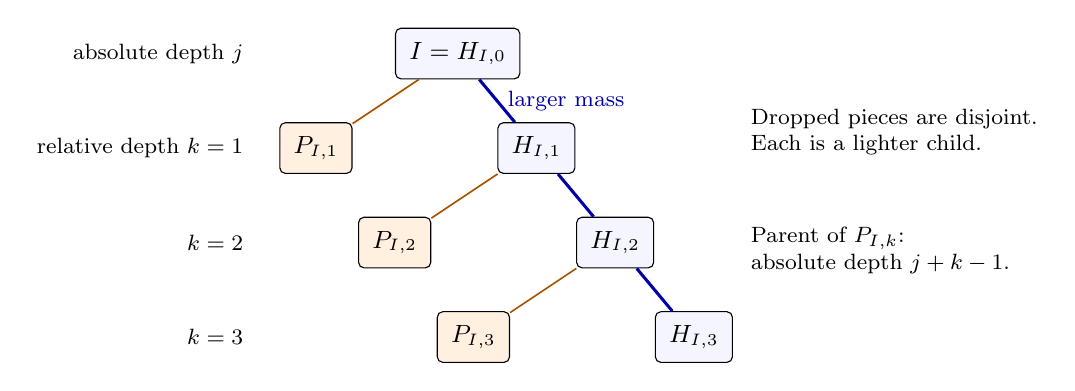
\begin{tikzpicture}[
  interval/.style={draw,rounded corners=2pt,inner sep=5pt,
                   fill=blue!4,font=\small},
  lighter/.style={draw,rounded corners=2pt,inner sep=5pt,
                  fill=orange!12,font=\small},
  heavyedge/.style={line width=1.1pt,blue!65!black},
  lightedge/.style={line width=.6pt,orange!65!black},
  note/.style={font=\footnotesize,align=left}
]
\node[interval] (root) at (0,0) {$I=H_{I,0}$};
\node[lighter] (p1) at (-1.8,-1.2) {$P_{I,1}$};
\node[interval] (h1) at (1.0,-1.2) {$H_{I,1}$};
\node[lighter] (p2) at (-.8,-2.4) {$P_{I,2}$};
\node[interval] (h2) at (2.0,-2.4) {$H_{I,2}$};
\node[lighter] (p3) at (.2,-3.6) {$P_{I,3}$};
\node[interval] (h3) at (3.0,-3.6) {$H_{I,3}$};
\draw[lightedge] (root)--(p1);
\draw[heavyedge] (root)--node[right,note] {larger mass}(h1);
\draw[lightedge] (h1)--(p2);
\draw[heavyedge] (h1)--(h2);
\draw[lightedge] (h2)--(p3);
\draw[heavyedge] (h2)--(h3);
\node[note,anchor=east] at (-2.6,0) {absolute depth $j$};
\node[note,anchor=east] at (-2.6,-1.2) {relative depth $k=1$};
\node[note,anchor=east] at (-2.6,-2.4) {$k=2$};
\node[note,anchor=east] at (-2.6,-3.6) {$k=3$};
\node[note,anchor=west] at (3.6,-1.0)
  {Dropped pieces are disjoint.\\
   Each is a lighter child.};
\node[note,anchor=west] at (3.6,-2.5)
  {Parent of $P_{I,k}$:\\
   absolute depth $j+k-1$.};
\end{tikzpicture}
\caption{Three steps of the heavier-child path.  At each step the
 lighter sibling is set aside; the chosen child is split again.  The
 dropped siblings together with the terminal child partition $I$.
 For fixed relative depth $k$, changing the frequency index $j$ changes
 the absolute depth of the parent.  This makes the parents distinct in
 the sum controlled by the convexity deficit.}
\label{fig:endpoint-tree}
\end{figure}


By additivity of $G_N$ and the triangle inequality in frequency $L^2$,
followed by \eqref{eq:endpoint-interpolated-dual},
\[
 e_j(I)^{1/2}
 \le C\sum_{k=1}^j2^{-k/6}m_{P_{I,k}}^{\alpha/2}
          +C2^{-j/6}m_{H_{I,j}}^{\alpha/2}.
\]
Use Cauchy--Schwarz with weights $2^{-k/6}$, including one additional
terminal weight $2^{-j/6}$.  Their sum is bounded independently of $j$.
Since $m_{H_{I,j}}\le m_I$, we obtain
\begin{equation}
 e_j(I)\le C\sum_{k=1}^j2^{-k/6}m_{P_{I,k}}^\alpha
                    +C2^{-j/6}m_I^\alpha.
 \label{eq:endpoint-heavy-path}
\end{equation}

We give the convexity calculation behind the sum of the first terms.
If a parent has child masses $a\ge b\ge0$, then
\begin{equation}
 (a+b)^\alpha-a^\alpha-b^\alpha
       \ge(2^\alpha-2)b^\alpha.
 \label{eq:endpoint-convexity-deficit}
\end{equation}
For $b>0$, divide by $b^\alpha$ and put $u=a/b\ge1$.
The function $(u+1)^\alpha-u^\alpha-1$ is increasing for $u\ge1$,
so its minimum is $2^\alpha-2$; the case $b=0$ is immediate.
Summing parent-minus-children deficits through depth $d-1$ telescopes to
\[
 m_{[0,1)}^\alpha-\sum_{Q\in\mathcal D_d}m_Q^\alpha
       \le m_{[0,1)}^\alpha.
\]
The deficits are nonnegative.  Letting $d\to\infty$ shows that the sum of
the lighter-child $\alpha$-powers over any collection of distinct dyadic
parents is at most
$m_{[0,1)}^\alpha/(2^\alpha-2)$.

Now fix $k\ge1$ and range over all $j\ge k$ and all
$I\in\mathcal D_j$.  The parent of $P_{I,k}$ is $H_{I,k-1}$, at absolute
depth $j+k-1$.  Different $j$ give different absolute depths; for the
same $j$, different $I$ have disjoint descendants.  These parents are
therefore distinct.  Consequently,
\[
 \sum_{j\ge k}\sum_{I\in\mathcal D_j}m_{P_{I,k}}^\alpha
      \le \frac{m_{[0,1)}^\alpha}{2^\alpha-2}.
\]
For the terminal terms, superadditivity of the $\alpha$th power gives
$\sum_{I\in\mathcal D_j}m_I^\alpha\le m_{[0,1)}^\alpha$.  Thus summing
\eqref{eq:endpoint-heavy-path}, first at fixed $k$ and then in $k$, gives
\[
 \sum_{j\ge1}\sum_{I\in\mathcal D_j}e_j(I)
 \le C m_{[0,1)}^\alpha
       \left(\sum_{k\ge1}2^{-k/6}+\sum_{j\ge1}2^{-j/6}\right)
 \le C.
\]
All sums are of nonnegative terms, so these rearrangements also follow
from finite truncations.  Finally apply
Lemma~\ref{lem:endpoint-time-separation} and sum its $O(2^{-2j})$ errors.
\end{proof}

\begin{remark}
The strict inequality $p>2$ is used quantitatively here:
$\alpha=3/2-1/p>1$ and $2^\alpha-2>0$.  At $p=2$ the convexity deficit
in \eqref{eq:endpoint-convexity-deficit} vanishes.  The gain in the time
tree therefore cannot be recovered merely from a weak $L^2$ version of
\eqref{eq:src24}.
\end{remark}

\begin{theorem}[Local strong maximal estimate]
\label{thm:maximal}
There is a constant $C$ such that, for every $f\in H^{1/3}(\R^2)$ whose
Fourier transform has compact support and every $x_0\in\R^2$,
\begin{equation}
 \int_{B(x_0,1)}\sup_{0\le t<1}|S(t)f(x)|\,dx
       \le C\|f\|_{H^{1/3}}.
 \label{eq:endpoint-strong-maximal}
\end{equation}
For arbitrary $f\in H^{1/3}(\R^2)$ there is a jointly measurable
representative $v_f(x,t)$, $0\le t<1$, continuous in $t$ for almost every
$x$, equal to $S(t)f$ as an $L^2$ function for each fixed $t$, and satisfying
the same bound with $S(t)f(x)$ replaced by $v_f(x,t)$.
\end{theorem}

\begin{proof}
First suppose $\widehat f$ has compact support.  Take a smooth frequency
partition
\[
 \psi_0+\sum_{j\ge1}\psi_j=1,
\]
where $\psi_0$ is supported in a fixed ball and $\psi_j$ is supported on
an annulus $|\xi|\asymp2^j$, with uniformly bounded overlap.  Put
$\widehat f_j=\psi_j\widehat f$.  Choose enlarged smooth annular cutoffs
$\chi_{2^j}$ equal to one on $\supp\psi_j$.  These are the cutoffs used in
Lemma~\ref{lem:endpoint-square-sum}.

For any common graph $t(x)$ and phase $w(x)$, Fourier inversion and the
definition of $G_N$ give
\[
 \int_\Omega w(x)\sum_{j\ge1}S(t(x))f_j(x)\,dx
       =(2\pi)^{-2}\sum_{j\ge1}
             \int\widehat f_j(\xi)G_{2^j}([0,1))(\xi)\,d\xi.
\]
Only finitely many summands are nonzero.  Cauchy--Schwarz in frequency
and in $j$ bounds the modulus by
\begin{align}
 C\left(\sum_{j\ge1}2^{2j/3}\|\widehat f_j\|_2^2\right)^{1/2}
  \left(\sum_{j\ge1}2^{-2j/3}
              \|G_{2^j}([0,1))\|_2^2\right)^{1/2}
 &\le C\|f\|_{H^{1/3}}.
 \label{eq:endpoint-frequency-cauchy-schwarz}
\end{align}
The first factor is bounded by the Sobolev square norm because on the
support of $\psi_j$ one has
$2^{2j/3}\asymp(1+|\xi|^2)^{1/3}$, and the supports overlap boundedly.
The second factor is bounded by \eqref{eq:endpoint-square-sum}.
The low-frequency term satisfies
$\sup_{x,t}|S(t)f_0(x)|\le C\|f_0\|_2$ by Cauchy--Schwarz on its fixed
frequency ball, so its integral over $\Omega$ has the same bound.

To recover the maximal function, take any finite list of times in
$[0,1)$ and let $t(x)$ be the first time attaining the maximal modulus
of $S(t)f(x)$ on that list.  Set
$w(x)=\overline{S(t(x))f(x)}/|S(t(x))f(x)|$ where the denominator is
nonzero, and set $w(x)=0$ otherwise.  These are measurable choices, and
the linearized integral is exactly the integral of the finite maximum.
Increase the list to a countable dense subset of $[0,1)$ containing zero.
Continuity in time and monotone convergence prove
\eqref{eq:endpoint-strong-maximal}.  The estimates above used only fixed
ball radii and spatial differences, so the constant is uniform in $x_0$.

For general $f$, choose $f_n$ with $\widehat f_n\in C_c^\infty(\R^2)$
and $\|f_n-f\|_{H^{1/3}}\le2^{-n}$.  In particular,
\[
 \sum_{n\ge1}\|f_{n+1}-f_n\|_{H^{1/3}}<\infty.
\]
Define the measurable functions
\[
 d_n(x)=\sup_{0\le t<1}
              |S(t)f_{n+1}(x)-S(t)f_n(x)|.
\]
The supremum can be taken over rational times, together with zero.
By \eqref{eq:endpoint-strong-maximal},
\[
 \sup_{x_0\in\R^2}\int_{B(x_0,1)}\sum_{n\ge1}d_n(x)\,dx
 \le C\sum_{n\ge1}\|f_{n+1}-f_n\|_{H^{1/3}}<\infty.
\]
A countable covering of $\R^2$ by unit balls therefore gives a single
full-measure set $E_0$ on which $\sum_n d_n(x)<\infty$.  For each
$x\in E_0$ the sequence $S(t)f_n(x)$ converges uniformly over
$0\le t<1$.  Denote its limit by $v_f(x,t)$, and define $v_f(x,t)=0$ for
$x\notin E_0$.  It is jointly measurable, and its time dependence is
continuous at every point of $E_0$, as a uniform limit of continuous
functions.

For each fixed $t$, unitarity gives $S(t)f_n\to S(t)f$ in $L^2$.
The pointwise limit on $E_0$ must therefore agree almost everywhere with
that $L^2$ limit.  This identifies the $L^2$ class of $v_f(\cdot,t)$ for
every fixed $t$; it does not assert a pointwise intersection over
uncountably many times.  Finally, Fatou's lemma in the maximal estimate
gives
\[
 \int_{B(x_0,1)}\sup_{0\le t<1}|v_f(x,t)|\,dx
    \le C\lim_{n\to\infty}\|f_n\|_{H^{1/3}}
    =C\|f\|_{H^{1/3}}.
\]
\end{proof}

\subsection{Recovering the Gaussian-first, all-real-time limit}

Fix $f\in H^{1/3}(\R^2)$ and the approximants just constructed, and write
$v=v_f$.  The same argument gives error envelopes with both pointwise
decay and spatial control at infinity.  Namely, let
\begin{equation}
 M_n(x)=\sup_{0\le t<1}|v(x,t)-S(t)f_n(x)|.
 \label{eq:endpoint-error-envelope}
\end{equation}
These functions are measurable by the rational-time supremum, since
the chosen $v(x,\cdot)$ is continuous even on the complement where it was
defined to be zero.  On $E_0$ the convergence is uniform, so
$M_n(x)\to0$.  Applying \eqref{eq:endpoint-strong-maximal} to
$f_\ell-f_n$ and then using Fatou yields
\begin{equation}
 \sup_{x_0\in\R^2}\int_{B(x_0,1)}M_n(x)\,dx
       \le C\|f-f_n\|_{H^{1/3}}.
 \label{eq:endpoint-envelope-local-mass}
\end{equation}
In particular, every $M_n$ is locally integrable with uniformly bounded
integrals over all translated unit balls.  This uniformity controls
Gaussian convolution far from its evaluation point.

\begin{lemma}[Gaussian approximation with uniform local mass]
\label{lem:endpoint-heat-envelope}
Let $h\ge0$ be locally integrable on $\R^2$ and suppose
\[
 A=\sup_{z\in\R^2}\int_{B(z,1)}h(y)\,dy<\infty.
\]
For $a>0$ let
\[
 K_a(z)=\frac1{4\pi a}e^{-|z|^2/(4a)}.
\]
Then $(K_a*h)(x)$ is finite for every $a>0$ and every $x$.  At every
Lebesgue point $x$ of $h$,
\begin{equation}
 \lim_{a\downarrow0}(K_a*h)(x)=h(x).
 \label{eq:endpoint-heat-envelope-limit}
\end{equation}
\end{lemma}

\begin{proof}
For a fixed $\rho>0$, cover each annulus
$2^\ell\rho\le |z|<2^{\ell+1}\rho$ by at most
$C(1+2^\ell\rho)^2$ unit balls.  Positivity gives
\begin{align}
 \int_{|z|\ge\rho}K_a(z)h(x-z)\,dz
 &\le \frac{CA}{a}\sum_{\ell\ge0}(1+2^\ell\rho)^2
                       e^{-4^\ell\rho^2/(4a)}\notag\\
 &\le C_\rho A a^{-1}e^{-\rho^2/(8a)},
 \qquad 0<a\le\min\{1,\rho^2\}.
 \label{eq:endpoint-gaussian-tail}
\end{align}
The series in the first line is finite for every fixed $a>0$.  Together
with local integrability this proves finiteness of the convolution, and
the second line shows that its distant contribution tends to zero.

At a Lebesgue point $x$, put
$H_x(r)=\int_{|z|<r}|h(x-z)-h(x)|\,dz=o(r^2)$.
Given $\varepsilon>0$, choose $\rho>0$ so that
$H_x(r)\le\varepsilon r^2$ for $0<r\le\rho$.  With
$k_a(r)=(4\pi a)^{-1}e^{-r^2/(4a)}$, radial integration by parts gives
\begin{align*}
 \int_{|z|<\rho}K_a(z)|h(x-z)-h(x)|\,dz
 &=k_a(\rho)H_x(\rho)
       +\int_0^\rho(-k_a'(r))H_x(r)\,dr\\
 &\le\varepsilon\left(k_a(\rho)\rho^2
                  +\int_0^\rho(-k_a'(r))r^2\,dr\right)
 \le C\varepsilon.
\end{align*}
Outside this neighborhood, \eqref{eq:endpoint-gaussian-tail} controls
the $h$ term, and the constant $h(x)$ is controlled by the vanishing
Gaussian mass outside $B(0,\rho)$.  Let $a\downarrow0$ and then
$\varepsilon\downarrow0$.
\end{proof}

\begin{proof}[Proof of Theorem~\ref{thm:main}]
At time zero, the fixed-time $L^2$ identification in
Theorem~\ref{thm:maximal} gives $v(\cdot,0)=f$ in $L^2$.  Since $f^*$
represents the same $L^2$ function on the set of Lebesgue points of $f$,
intersect $E_0$ with the full-measure set where $v(x,0)=f^*(x)$ and
with that Lebesgue-point set.
Next intersect with the Lebesgue-point sets of the countably many
functions $M_n$.  Call the resulting full-measure set $E$.  For every
$x\in E$ we now have, simultaneously,
\begin{equation}
 \begin{gathered}
 v(x,\cdot)\text{ is continuous on }[0,1),\qquad v(x,0)=f^*(x),\\
 M_n(x)\longrightarrow0,\qquad
 (K_a*M_n)(x)\longrightarrow M_n(x)
       \quad\text{as }a\downarrow0\text{ for every }n.
 \end{gathered}
 \label{eq:endpoint-common-good-set}
\end{equation}
The last assertion follows from
\eqref{eq:endpoint-envelope-local-mass} and
Lemma~\ref{lem:endpoint-heat-envelope}.  Only countably many exceptional
sets were removed.

For each fixed $t\in[0,1)$, the function $v(\cdot,t)$ represents
$S(t)f$ in $L^2$.  Since $K_a(x-\cdot)\in L^2$, convolution at a given
$x$ is an $L^2$ pairing and is independent of the representative of this
$L^2$ class.  Plancherel's identity therefore gives
\begin{equation}
 (K_a*v(\cdot,t))(x)
  =\frac1{(2\pi)^2}\int e^{ix\cdot\xi-it|\xi|^2-a|\xi|^2}
                                \widehat f(\xi)\,d\xi
  =U_af(x,t)
 \label{eq:endpoint-exact-convolution}
\end{equation}
for every $x\in\R^2$, every $a>0$, and every $0<t<1$.
The integral is absolutely convergent by Cauchy--Schwarz.  The
quantifiers in this step are significant: for each arbitrary $t$, an
identity of $L^2$ classes gives the convolution identity at every
evaluation point.  There is no intersection of time-dependent pointwise
exceptional sets in \eqref{eq:endpoint-exact-convolution}.

For the approximants, absolute Fourier integrability yields
\begin{align}
 R_n(a)&:=\sup_{x\in\R^2,\,0<t<1}
               |U_af_n(x,t)-S(t)f_n(x)|\notag\\
 &\le\frac1{(2\pi)^2}\int
               |1-e^{-a|\xi|^2}|\,|\widehat f_n(\xi)|\,d\xi
       \longrightarrow0\qquad(a\downarrow0).
 \label{eq:endpoint-smooth-heat-limit}
\end{align}
Positivity of $K_a$, the error envelope, and
\eqref{eq:endpoint-exact-convolution} give, for each $x\in E$,
\begin{equation}
 \sup_{0<t<1}|U_af(x,t)-v(x,t)|
 \le (K_a*M_n)(x)+M_n(x)+R_n(a).
 \label{eq:endpoint-uniform-gaussian-comparison}
\end{equation}
Indeed the difference between the two convolutions is bounded by
$K_a*M_n$, because
$|v(y,t)-S(t)f_n(y)|\le M_n(y)$ for almost every $y$, simultaneously for
all $t$; the remaining two differences are bounded by $R_n(a)$ and
$M_n(x)$.  All these convolutions are finite by the preceding lemma or
by the $L^2$ pairing.

Fix $n$ and take $\limsup_{a\downarrow0}$ in
\eqref{eq:endpoint-uniform-gaussian-comparison}.  By
\eqref{eq:endpoint-common-good-set} and
\eqref{eq:endpoint-smooth-heat-limit},
\[
 \limsup_{a\downarrow0}\sup_{0<t<1}|U_af(x,t)-v(x,t)|
        \le2M_n(x).
\]
Let $n\to\infty$.  Thus for every $x\in E$,
\begin{equation}
 \lim_{a\downarrow0}\sup_{0<t<1}|U_af(x,t)-v(x,t)|=0.
 \label{eq:endpoint-uniform-gaussian-limit}
\end{equation}
In particular, at each such $x$ the finite limit defining $u_f(x,t)$
exists for every real $0<t<1$, with $t$ fixed before $a$ tends to zero,
and it equals $v(x,t)$.  Continuity at zero now gives
\[
 \lim_{\substack{t\downarrow0\\t\in\R}}u_f(x,t)
     =\lim_{t\downarrow0}v(x,t)=v(x,0)=f^*(x).
\]
This proves Theorem~\ref{thm:main}.
\end{proof}
